\section{Implementation Details}\label{sec:appendix-implementation}

\subsection{Training Data} \label{sec:appendix-data}

We curate a multi-source training mixture that covers text, image, video, and visually-rich document retrieval.
The composition ratio for each data source is shown in~\autoref{fig:training-data-pie}, and per-dataset retrieval instructions are listed in~\autoref{tab:train_instructions_text} and~\autoref{tab:train_instructions_multimodal}.

\begin{wrapfigure}{r}{0.4\linewidth}
\centering
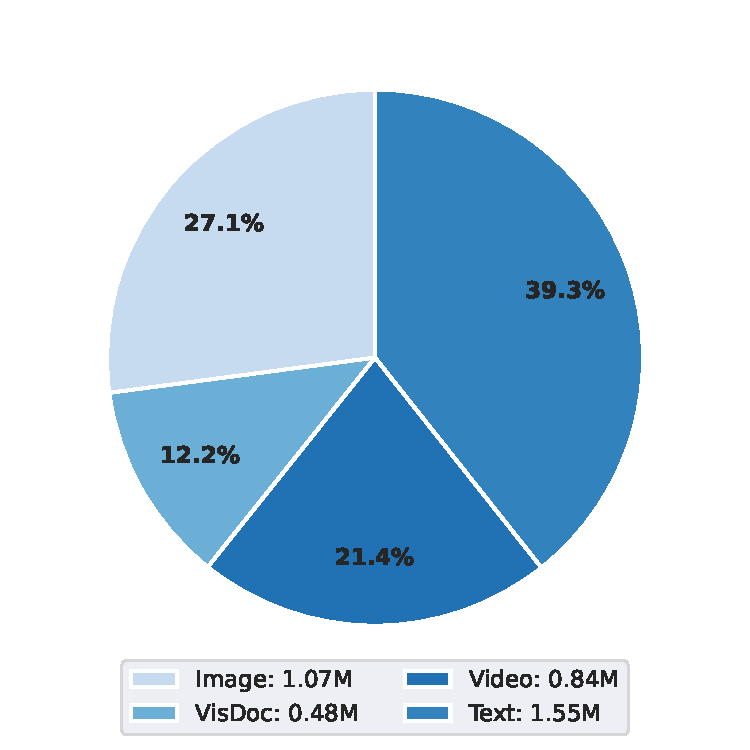
\includegraphics[width=\linewidth]{resources/training_data_pie.pdf}
\caption{Distribution of training data sources.}
\label{fig:training-data-pie}
\end{wrapfigure}

\paragraph{Text Training Data.}
To enable text embedding capabilities, we include training pairs from Echo-Embedding~\citep{echoemb} and M3-Embedding~\citep{bgem3}.
The text subset comprises NLI, DuReader, ELI5, FEVER, HotpotQA, MIRACL, MrTyDi, MSMARCO Passage, MSMARCO Document, Natural Questions, Quora Duplicates, SQuAD, T2Ranking, TriviaQA, and MLDR.
For standard text tasks we set a maximum sequence length of 1{,}500 tokens; for long-document retrieval (MLDR) we extend this to 1{,}800 tokens.



\paragraph{Multimodal Training Data.}
For video retrieval, we utilize VideoCaption300k and VideoQA240k from LLaVA-Hound~\citep{llava-hound}.
We sample 8 frames per video and allocate up to 200 tokens per frame.
For visual document retrieval, we incorporate ColPali train (118k), VisRAG-Synthetic (239k), and VisRAG-IID (123k) from ViDoRe~\citep{vidore} and VisRAG~\citep{visrag}.
For image-text retrieval, we include the MMEB training datasets~\citep{vlm2vec}, covering CIRR, NIGHTS, MSCOCO, VisualNews, N24News, ImageNet-1K, SUN397, VOC2007, HatefulMemes, A-OKVQA, OK-VQA, Visual7W, ChartQA, DocVQA, InfographicsVQA, VisDial, and WebQA.
For video tasks, the maximum sequence length is 1{,}800 tokens with 8 frames sampled per video and up to 200 tokens per frame.
For all other multimodal tasks, the maximum sequence length is 1{,}500 tokens, with up to 1{,}000 tokens allocated to the image. 
\begin{figure*}[htbp]
\centering
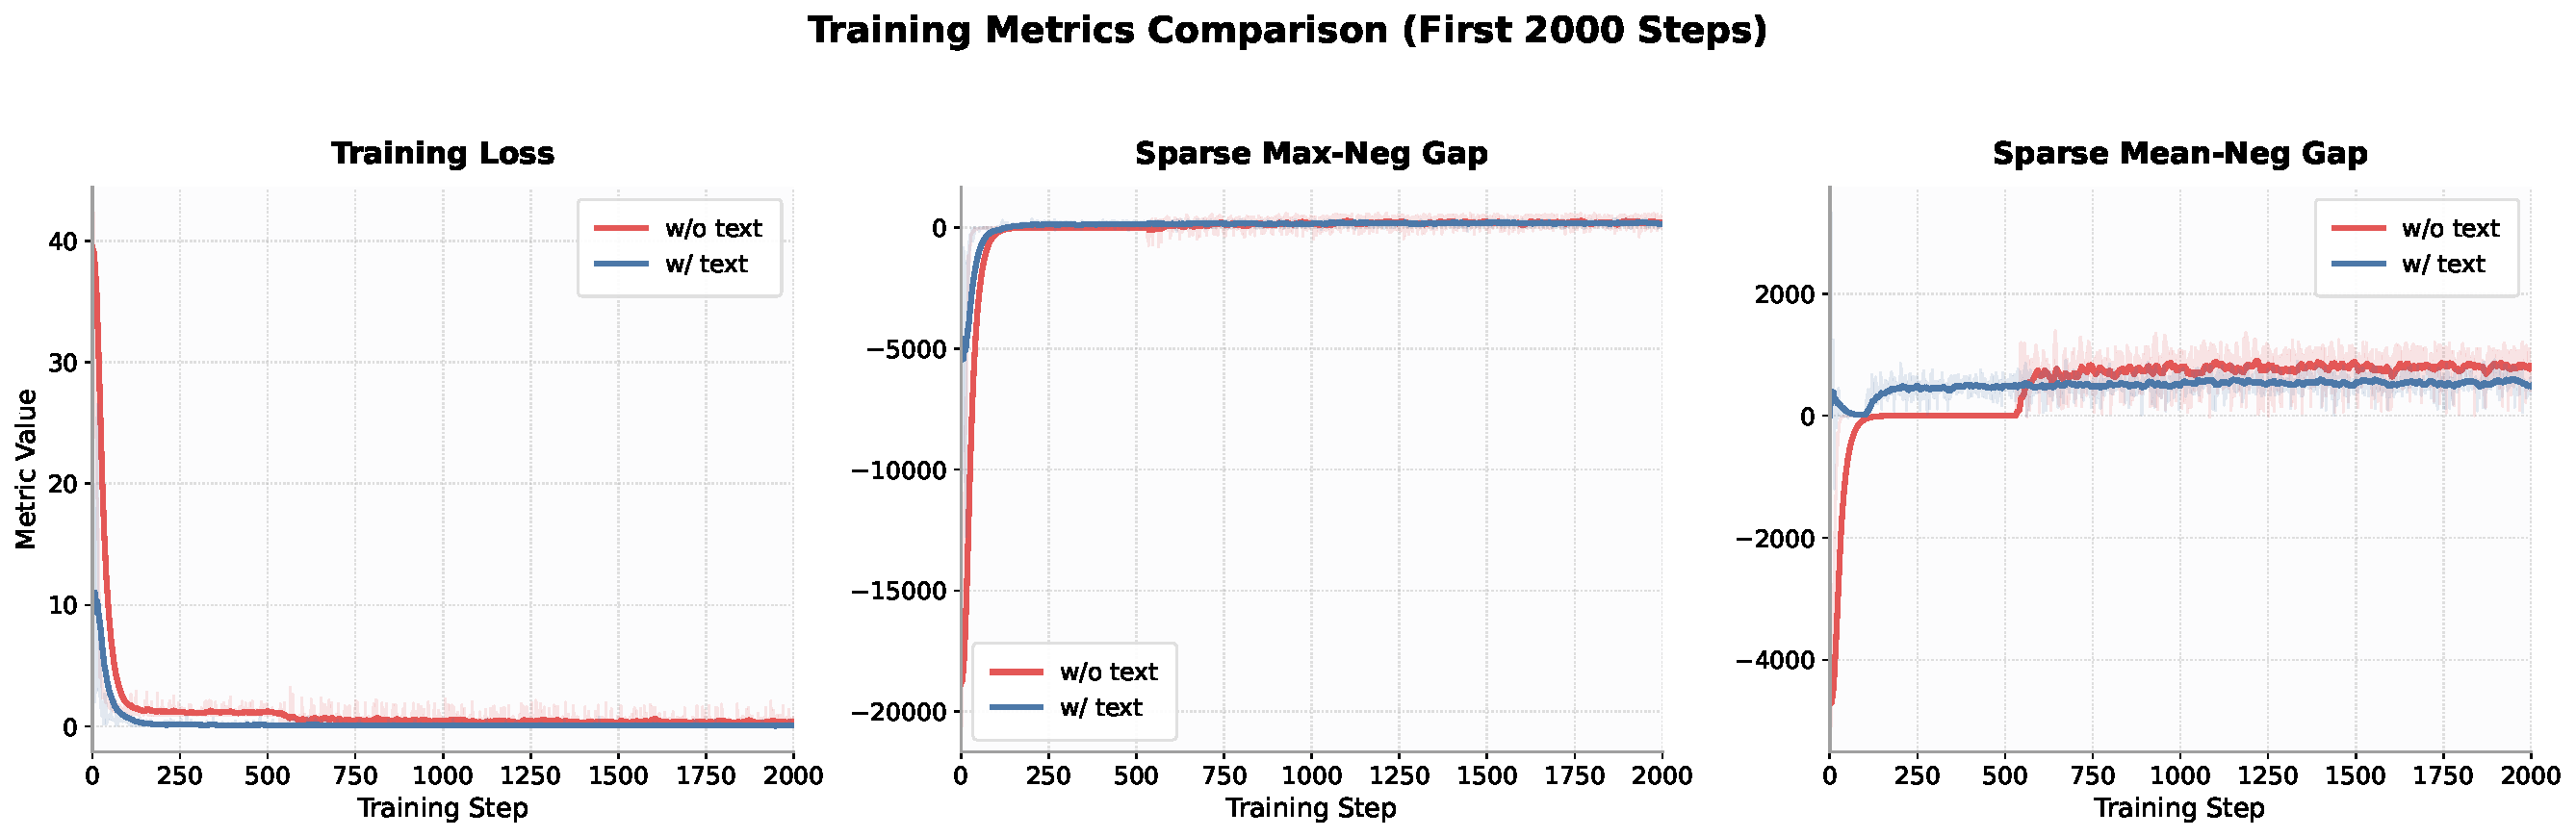
\includegraphics[width=0.9\linewidth]{resources/combined_training_metrics.pdf}
\caption{Training dynamics comparison. We plot the loss, max negative gap, and mean negative gap during training. }
\label{fig:training-metrics}
\end{figure*}

\begin{table*}[htbp]
\centering
\begin{tabularx}{0.9\textwidth}{p{3.5cm} X}
\toprule[.1em]
\textbf{Dataset} & \textbf{Instruction} \\
\midrule
AllNLI & Given a premise, retrieve a hypothesis that is entailed by the premise. Retrieve semantically similar text. \\
DuReader & Given a Chinese search query, retrieve web passages that answer the question. \\
ELI5 & Provided a user question, retrieve the highest voted answers on Reddit ELI5 forum. \\
FEVER & Given a claim, retrieve documents that support or refute the claim. \\
HotpotQA & Given a multi-hop question, retrieve documents that can help answer the question. \\
MIRACL & Given a question, retrieve Wikipedia passages that answer the question. \\
MrTyDi & Given a question, retrieve Wikipedia passages that answer the question. \\
MSMARCO-Doc & Given a web search query, retrieve relevant documents that answer the query. \\
MSMARCO-Psg & Given a web search query, retrieve relevant passages that answer the query. \\
NQ & Given a question, retrieve Wikipedia passages that answer the question. \\
Quora & Given a question, retrieve questions that are semantically equivalent to the input question. \\
SQuAD & Retrieve Wikipedia passages that answer the question. \\
T2Ranking & Given a Chinese search query, retrieve web passages that answer the question. \\
TriviaQA & Retrieve Wikipedia passages that answer the question. \\
MLDR & Retrieve Wikipedia passages that answer the question. \\
\bottomrule[.1em]
\end{tabularx}
\caption{Retrieval instructions for text training datasets.}
\label{tab:train_instructions_text}
\end{table*}

\subsection{Training Details}

We initialize from a pretrained multimodal backbone and add $N{=}16$ special tokens to the tokenizer and embedding matrix.
Training uses LoRA~\citep{lora2022} applied to the attention and MLP projections (\texttt{q\_proj}, \texttt{k\_proj}, \texttt{v\_proj}, \texttt{up\_proj}, \texttt{down\_proj}, \texttt{gate\_proj}), with the visual encoder frozen.
We train in \texttt{bf16} mixed precision with DeepSpeed ZeRO and gradient checkpointing enabled.


\paragraph{Hyperparameters.}
We train the \ours models based on Qwen3.5. 
We use a cosine learning rate schedule with a peak learning rate of $3{\times}10^{-5}$ and a warmup ratio of 0.1. 
The dense retrieval temperature is set to $\tau{=}0.03$, and the sparse retrieval temperature is $\tau_s{=}32$. 
For the FLOPS regularizer, we set $\alpha_q = \alpha_d = 1{\times}10^{-4}$ with a linear ramp-up over the first 200 steps. 
The sparse loss factor $\lambda{=}1.0$ balances the sparse and dense InfoNCE losses equally.
We train for 1 epoch and fix the random seed to 42. 
Training is conducted on 16$\times$A100 GPUs for \ours-2B and \ours-4B with a per-device batch size of 16, and on 32$\times$A100 GPUs for \ours-9B with a per-device batch size of 8, ensuring a consistent batch size of 256 across all models.

\subsection{Training Analysis}

Since sparse scores are computed via inner products, sparse training can be unstable due to the large dynamic range of unnormalized similarities.
We find that incorporating text training data significantly stabilizes and accelerates multimodal sparse model training.
Following GVE~\citep{gve}, we monitor three key metrics during training: loss, max negative gap, and mean negative gap. The max negative gap is defined as the largest score difference between a positive and the negative within a batch, while the mean negative gap is the average score difference across all positive-negative pairs in a batch. 
As shown in~\autoref{fig:training-metrics}, when trained with text data, the model learns effective sparse representations rapidly ($<$100 steps). In contrast, training exclusively on multimodal data (\eg image, video) requires nearly 500 steps before the model can reliably distinguish positives from negatives.



\begin{table*}[htbp]
\centering
\begin{tabularx}{\textwidth}{p{3cm} X}
\toprule[.1em]
\textbf{Dataset} & \textbf{Instruction} \\
\midrule
CIRR & Given an image, find a similar everyday image with the described changes. \\
NIGHTS & Find a day-to-day image that looks similar to the provided image. \\
MSCOCO & Select the portion of the image that isolates the object. \\
MSCOCO (image-to-text) & Find an image caption describing the given everyday image. \\
VisualNews (image-to-caption) & Find a caption for the news in the given photo. \\
MSCOCO (text-to-image) & Find me an everyday image that matches the given caption. \\
VisualNews (text-to-image) & Retrieve an image of this news caption. \\
N24News & Classify the domain of the given news image. \\
ImageNet\_1K & Classify the given image. \\
SUN397 & Identify the scene shown in the image. \\
VOC2007 & Identify the object shown in the image. \\
HatefulMemes & Determine whether the given image constitutes hateful speech or not. \\
A-OKVQA & Answer the question about the given image. \\
OK-VQA & Answer the question about the given image. \\
Visual7W & Answer the question about the given image. \\
ChartQA & Answer the question about the given chart image. \\
DocVQA & Answer the question about the given document image. \\
InfographicsVQA & Answer the question about the given infographic image. \\
VisDial & Retrieve an image based on the given dialogue. \\
WebQA & Find a Wikipedia image that answers this question. \\
VISRAG-IID & Find a Wikipedia image that answers this question. \\
ViDoRe & Find a Wikipedia image that answers this question. \\
VisRAG-Synthetic & Find a document image that answers this question. \\
VideoCaption300k (text-to-video) & Find a video that matches the given caption. \\
VideoCaption300k (video-to-text) & Find a caption that describes the given video. \\
VideoQA240k & Answer the question about the given video. \\
\bottomrule[.1em]
\end{tabularx}
\caption{Retrieval instructions for multimodal training datasets.}
\label{tab:train_instructions_multimodal}
\end{table*}